\documentclass[14pt]{beamer}
\usepackage[utf8]{inputenc}
\usepackage[T1]{fontenc}
\usepackage{lmodern}
\usepackage[english]{babel}
\usepackage{graphicx}
\usetheme{Boadilla}

\makeatletter
\def\verbatim{\small\@verbatim \frenchspacing\@vobeyspaces \@xverbatim}
\makeatother

\renewcommand{\texttt}[1]{{{\tt\color{blue}#1}}}


\begin{document}
	\author{Lukáš Růžička}
	\title{GIT -- krok za krokem}
	%\subtitle{}
	%\logo{}
%	\institute{Red Hat}
	\date{prosinec 2020}
	%\subject{}
	%\setbeamercovered{transparent}
	%\setbeamertemplate{navigation symbols}{}
	\begin{frame}[plain]
		\maketitle
	\end{frame}


	\begin{frame}{Co je GIT?}
	\begin{itemize}
		\item verzovací systém
		\item open source
		\item s aktivním vývojem
		\item vytvořil je Linus Torvalds
		\item distribuovaný (necentralizovaný)
	\end{itemize}
	\end{frame}


	\begin{frame}{Proč?}
	 Vytváření věcí duševní povahy často zahrnuje:
		\vspace{5pt}
		
	\begin{itemize}
		\item přepisování
		\item mazání
		\item zkoušení slepých cest
		\item návraty k předchozímu
		\item revize a korekce od spolupracovníků
	\end{itemize}
\end{frame}
		
\begin{frame}{Srovnání s kdysi}
	
	\begin{tabular}{l|l}
		\textbf{pravěk} & \textbf{gitvěk} \\
		\hline opište si zadání &  fork \\
		průběžně odevzdávejte & git commit \\
		zkus ještě další verzi & git branch \\
		použij obě verze, přepiš  & git merge \\
		tady jsou opravy, přepiš & git merge \\
		raději bych přece jen tu dřívější verzi & git reset \\
		zahoď to & git rm \\
        cos to zahodil, ty jelito? & git clone
	\end{tabular}
	
	\vspace{10pt}
		
	Prostě $\ldots${} \textbf{Vždycky GIT!}

\end{frame}

\begin{frame}{Co potřebujeme?}
	\begin{itemize}
		\item účet na nějakém serveru s gitem (Pagure, Github, Bitbucket, Atlasian)
		\item nainstalovaný git
		\item dobrý je i nějaký grafický Git editor (tig, gitk, gitg)
	\end{itemize}
\end{frame}

	\begin{frame}{Instalace Gitu}
		\begin{itemize}
		\item Fedora: sudo dnf install git
		\item Debian: sudo apt-get install git
		\item Mac: http://git-scm.com/download/mac
		\item Windows: http://git-scm.com/download/win
		\item github.com -- založit účet
		\end{itemize}
	\end{frame}

	\begin{frame}{Konfigurace gitu}
		\begin{itemize}
		\item \texttt{git config -\,-global user.name "Your Name"}
		\item \texttt{git config -\,-global user.email "yourname@example.com"}
		\end{itemize}
	\end{frame}

	\begin{frame}{Vytváříme první repozitář}
		\begin{enumerate}
		\item Běžte na stránku svého profilu.
		\item Klikněte na \textbf{Repositories}.
		\item Klikněte na \textbf{New}.
		\item Vyplňte údaje.
		\item Klikněte na \textbf{Create repository}.
		\end{enumerate}
	\end{frame}

	\begin{frame}{Stránka profilu}
        \begin{center}
        \frame{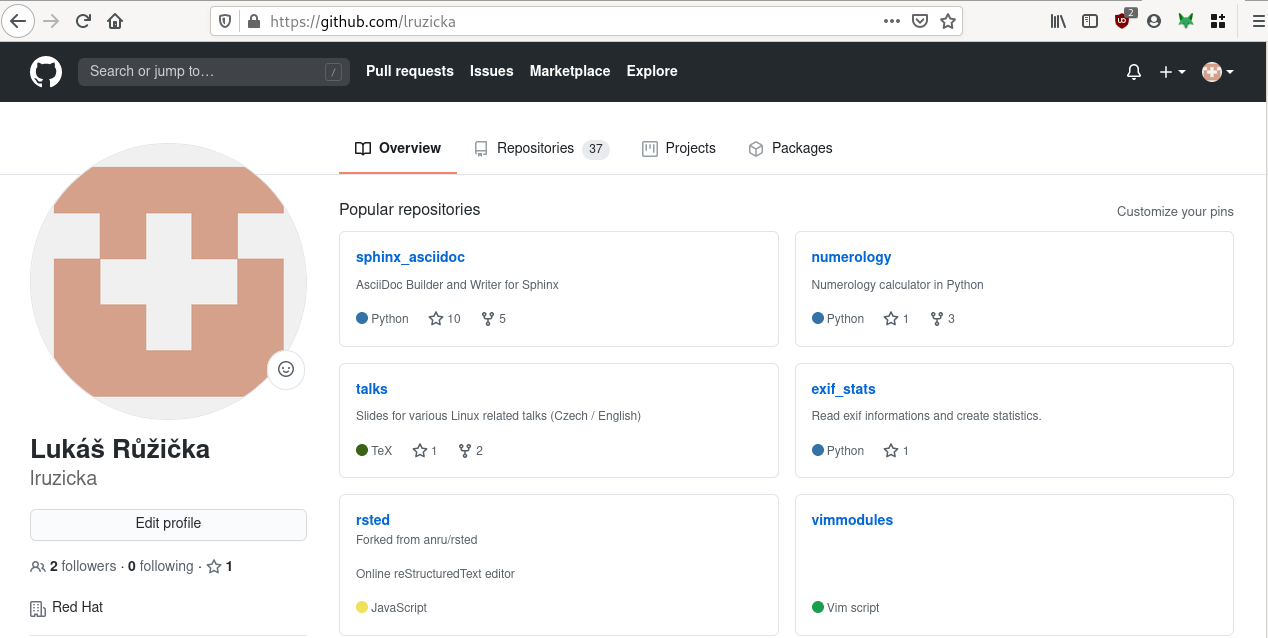
\includegraphics[width=10cm]{images/profil.png}}
        \end{center}
	\end{frame}

	\begin{frame}{Nový repozitář}
	\begin{center}
		\frame{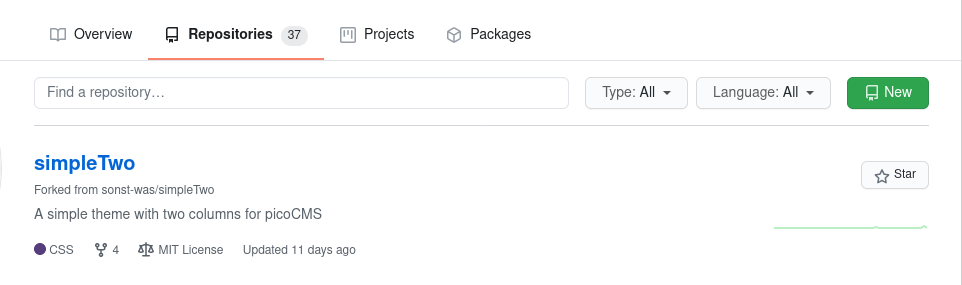
\includegraphics[width=10cm]{images/repositories.png}}
	\end{center}
	\end{frame}

	\begin{frame}{Vytvořit nový repozitář}
	\begin{center}
		\frame{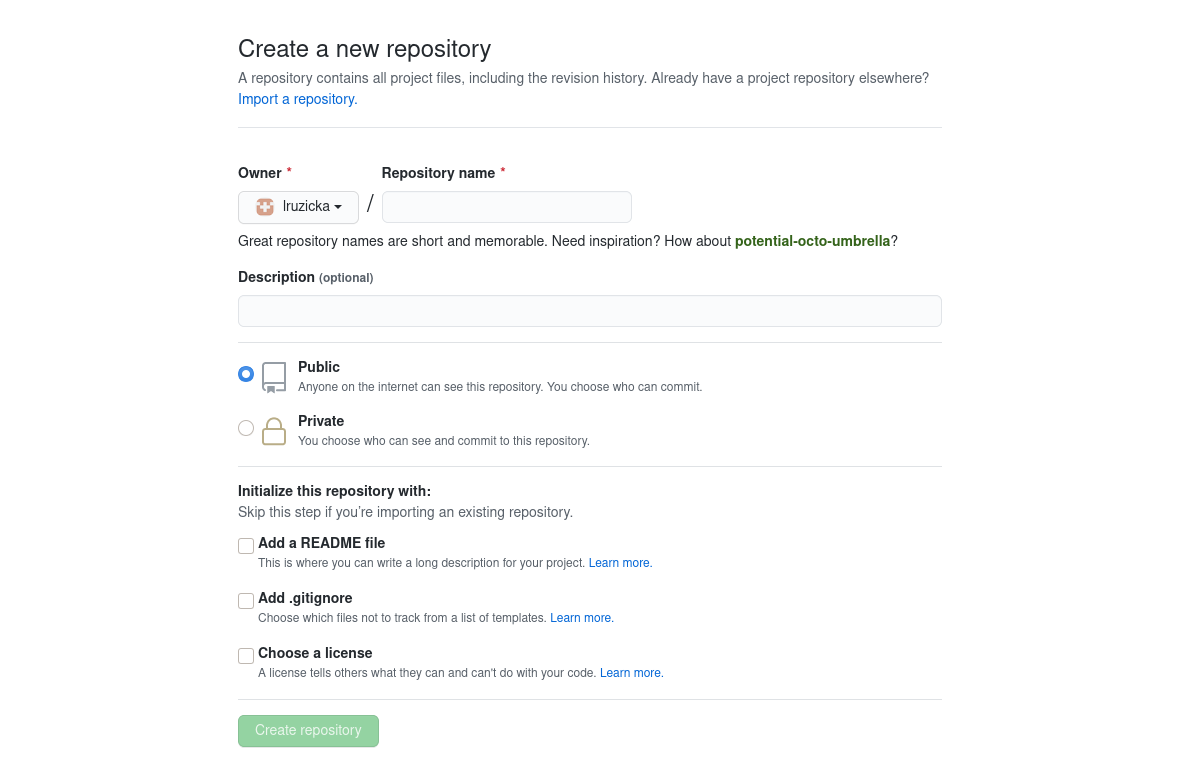
\includegraphics[width=10cm]{images/createnew.png}}
	\end{center}
	\end{frame}

	\begin{frame}{Klonovat repozitář}
		Kopírujeme repozitář k sobě na disk.
		\begin{enumerate}
		\item Přístup SSH klíčem \\ {\small \texttt{git clone git@github.com:lruzicka/hokuspokus.git}}
		\item Přístup heslem \\ \texttt{git clone {\small https://github.com/lruzicka/hokuspokus.git}}
	\end{enumerate}
	\end{frame}

	\begin{frame}{Iniciace repozitáře}
	Pokud nemůžeme z nějakého důvodu repozitář naklonovat, nebo chceme vytvořit pouze lokální repozitář (bez serveru), můžeme repozitář tzv. \textbf{založit} (initiate) příkazem
	\begin{itemize}
		\item \texttt{git init}
	\end{itemize}
	\end{frame}

	\begin{frame}{Zobrazení konkrétní situace}
	Zjišťujeme situaci na lokální kopii. Příkaz nám ukáže základní informace o repozitáři
	\begin{itemize}
		\item aktuální větev
		\item stav větve (aktuální, zaostává, předchází se)
		\item stav rozdělané práce
	\end{itemize}
	\end{frame}

	\begin{frame}{Zobrazení historie}
	Zobrazíme záznam \textbf{historie} pro aktuální větev daného repozitáře od nejnovějšího po nejstarší.
	\begin{itemize}
		\item commit (hash)
		\item autor commitu
		\item datum commitu
		\item název commitu (commit message)
		\item \texttt{git log -\,-oneline}
	\end{itemize}
	\end{frame}


	\begin{frame}{Prohlížení commitu}
	Zobrazíme obsah daného commitu.
	\begin{itemize}
		\item \texttt{git show HEAD$ \sim $2}
		\item \texttt{git show 622a1fee15c347}
	\end{itemize}
	\end{frame}

	\begin{frame}{Úprava obsahu}
		Obsah v gitu může být jakýkoliv, takže jej upravujeme patřičným způsobem, jak potřebujeme a jak jsme zvyklí.
			\begin{itemize}
			\item textový editor
			\item textový procesor
			\item specifická aplikace
		\end{itemize}
		Git si každé změny všimne.
	\end{frame}

	\begin{frame}{Untracked a Staging}
	Když provedeme nějaké úpravy, například přidáme soubor, git o něm neví a označuje ho jako \textbf{untracked}. Musíme o nich gitu říct. 
	
	Stejně tak úpravy prodevedené u známých souborů nejsou primárně zařazeny do zpracování, dokud to \textbf{explicitně neřekneme}. 
	
	Tento proces se nazývá \textbf{staging }. V analogii vlaku se jedná o \textit{rezervaci jízdenek}.
		\begin{itemize}
			\item \texttt{git add novy-soubor}
			\item \texttt{git add adresar/*}
			\item \texttt{git add .}
		\end{itemize}
	\end{frame}

	\begin{frame}{Zapsání obsahu do stromu}
	Ačkoliv jsme Git informovali o změnách, dokud je nezapíšeme do stromu
	historie, nejsou součástí vývojové větve.
	
	V analogii vlaku je potřeba do vlaku \textit{nastoupit}.

	\begin{itemize}
		\item \texttt{git commit}
		\item \texttt{git commit -m "Commit message"}
	\end{itemize}
	\end{frame}
	

	\begin{frame}{Nahrání na server}
		Lze samozřejmě Git používat pouze lokálně, ale chceme-li spolupracovat s dalšími lidmi, musíme naše změny nahrát na server.
	\begin{itemize}
		\item \texttt{git push}
	\end{itemize}
To lze pouze tehdy, když mezi lokální a serverovou kopii nejsou žádné \textbf{konflikty}.
	\end{frame}

	\begin{frame}{Synchronizace se serverem}
	Před každým zahájení práce je nutné stáhnout novinky ze serveru, aby se minimalizovalo riziko konfliktů.
	\begin{itemize}
		\item \texttt{git pull} (zkratka pro následující)
		\item \texttt{git fetch origin}
		\item \texttt{git rebase origin/branch} nebo
		\item \texttt{git merge origin/branch}
	\end{itemize}
	Použití jednotlivých strategií záleží na vkusu každého, jsou mezi nimi však určité rozdíly, které si ukážeme později.
	\end{frame}

	\begin{frame}{Práce s větvemi}
	Větve nám umožňují pracovat současně na projektu tak, abychom si navzájem nepřekáželi. 
	\begin{itemize}
		\item Git podporuje neomezené množství větví
		\item větve umožňují oddělenou práci
	\end{itemize}
	Použití jednotlivých strategií záleží na vkusu každého, jsou mezi nimi však určité rozdíly, které si ukážeme později.
	\end{frame}

	\begin{frame}{Příklad větvení}
		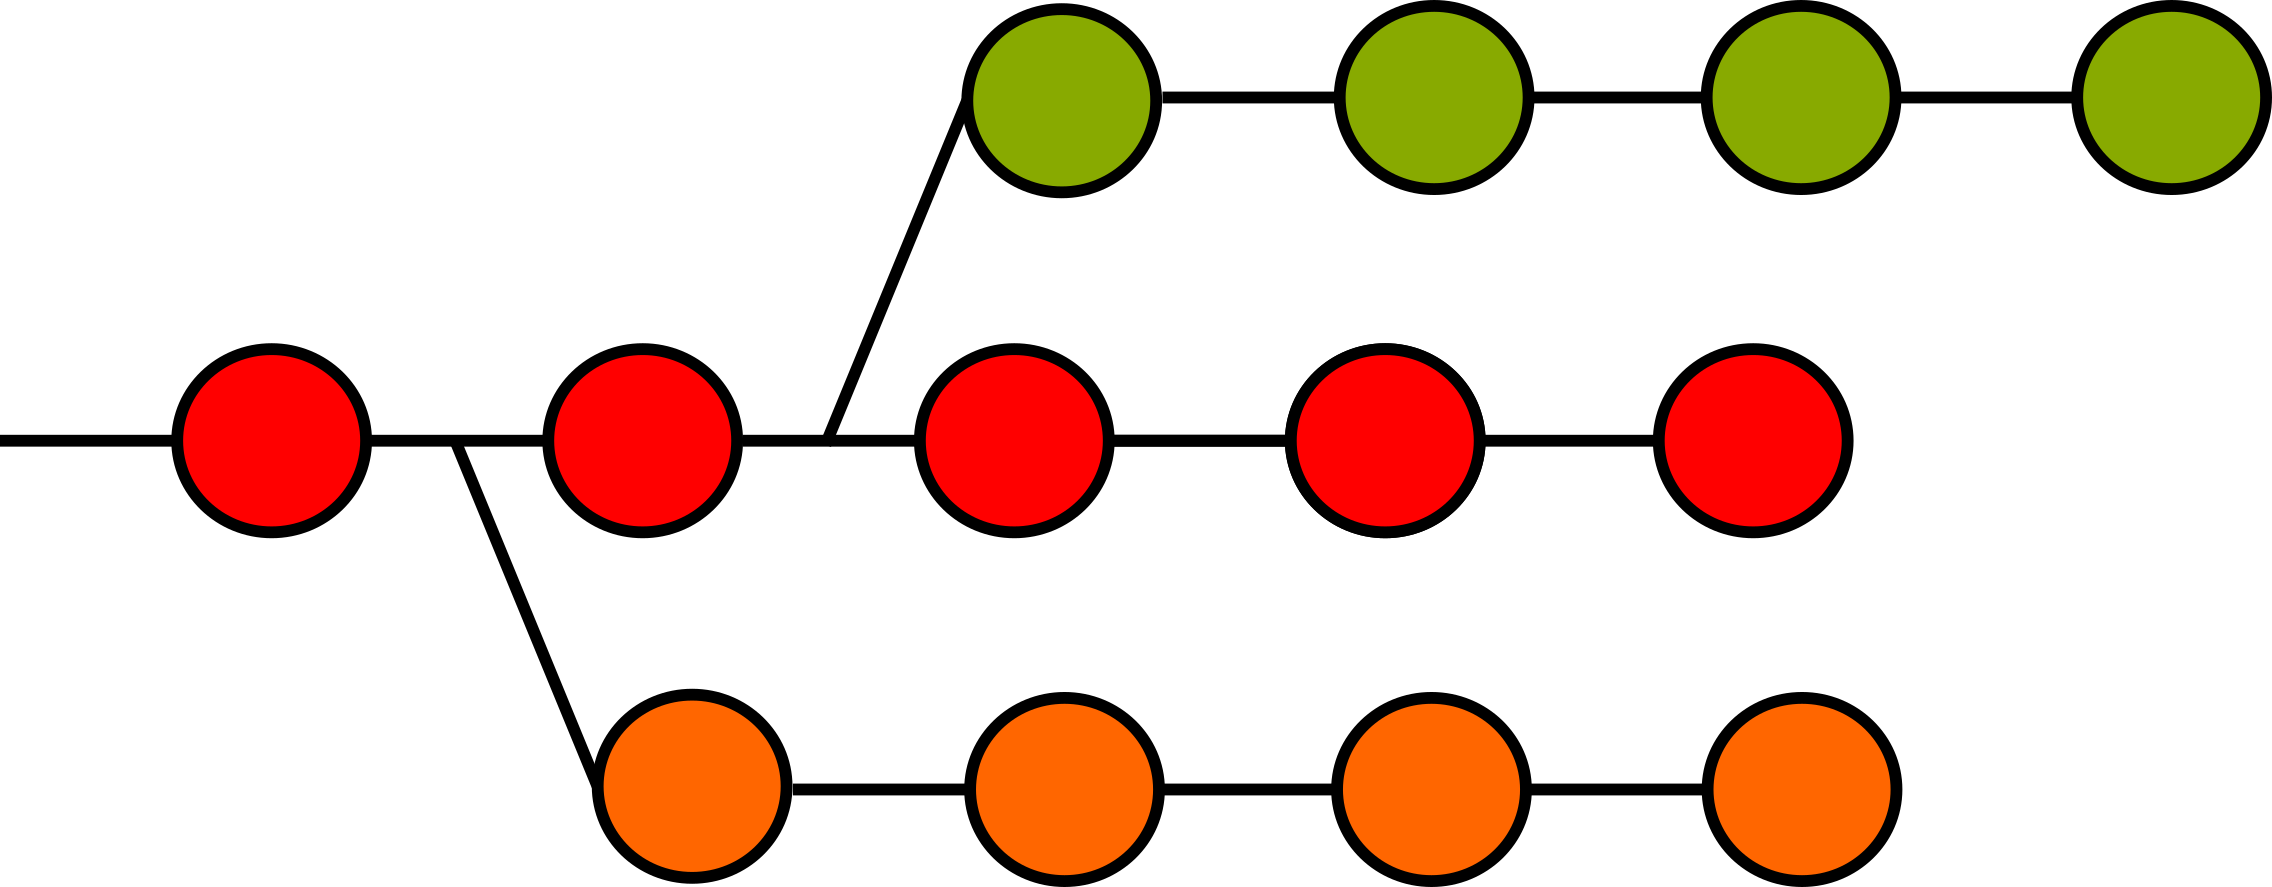
\includegraphics[width=10cm]{images/branches}
	\end{frame}

	\begin{frame}{Zobrazení všech větví projektu}
		\begin{enumerate}
			\item \texttt{git branch}
		\end{enumerate}
	\end{frame}

	\begin{frame}{Změna aktuální větve}
		Do existující větve se lze přepnout příkazem \textbf{checkout}. Přepnutí do neexistující větve (vytvoření nové) vyžaduje navíc přepínač \textbf{-b}.
	\begin{enumerate}
		\item \texttt{git checkout branch}
		\item \texttt{git checkout -b branch}
	\end{enumerate}
	Nová větev se obsahově shoduje s aktuální větví až do místa rozvětvení. Lze tedy hned po vyvětvení pokračovat v práci.
	\end{frame}

	\begin{frame}{Slučování větví}
	Větev můžeme sloučit s jinou větví a tak do jedné větve převzít obsah druhé větve, například do hlavní větve lze převzít vývoj nějakého doplňku z vedlejší větve. 
	
	Pro slučování větví existují dvě strategie:
	\begin{enumerate}
		\item merge (prorůstání)
		\item rebase (roubování)
	\end{enumerate}
	Slučování větví je možné pouze tehdy, když mezi větvemi \textbf{není konflikt}.

	\end{frame}

	\begin{frame}{Příklad prorůstání}
	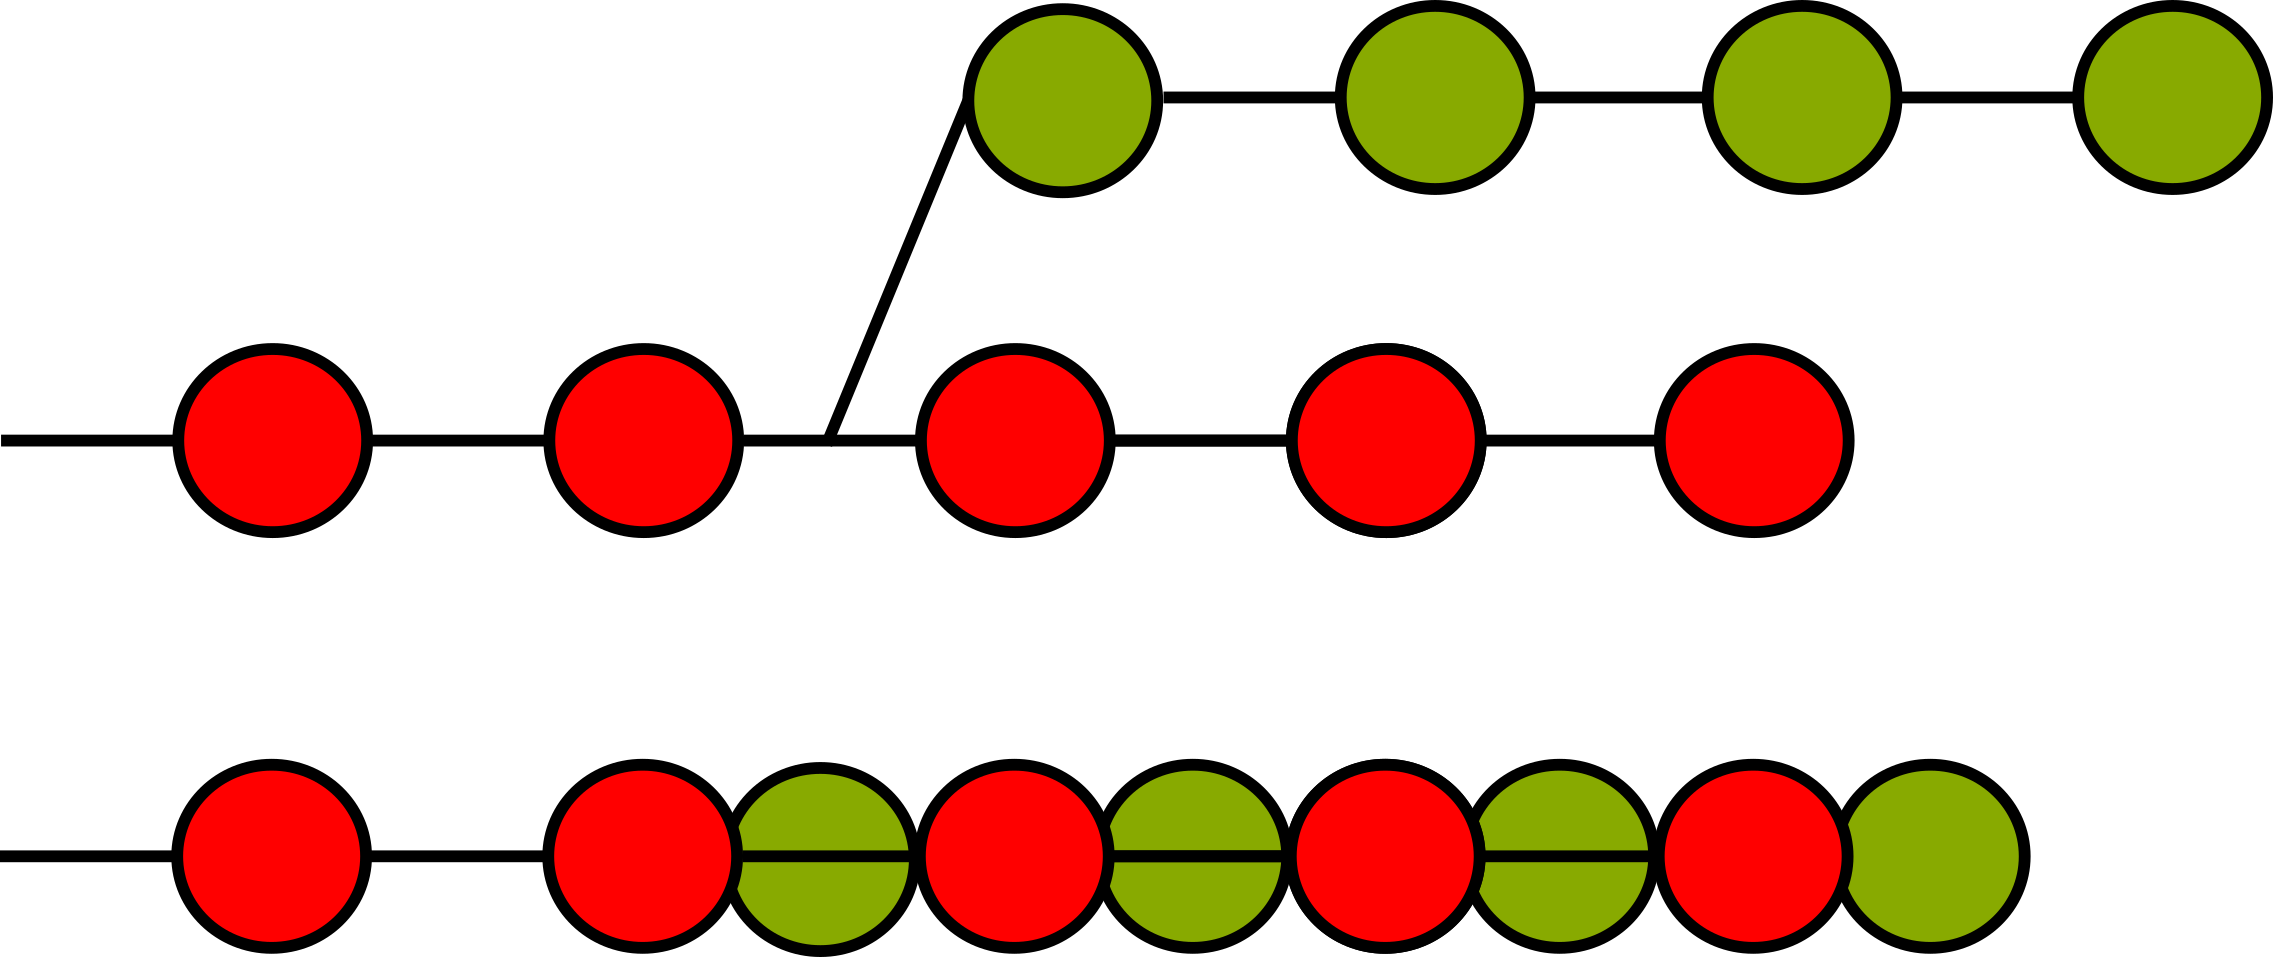
\includegraphics[width=10cm]{images/merge}
	\end{frame}

	\begin{frame}{Slučování větví - prorůstání}
	Větve sloučíme následujícím postupem.
	
	\begin{enumerate}
		\item Přepneme se do cílové větve, to je ta, do které chceme slučovat \\
		\texttt{git checkout target-branch}
		\item Sloučíme obsah zdrojové větve do cílové větve \\
		\texttt{git merge source-branch}
	\end{enumerate}
	\end{frame}

	\begin{frame}{Příklad roubování}
	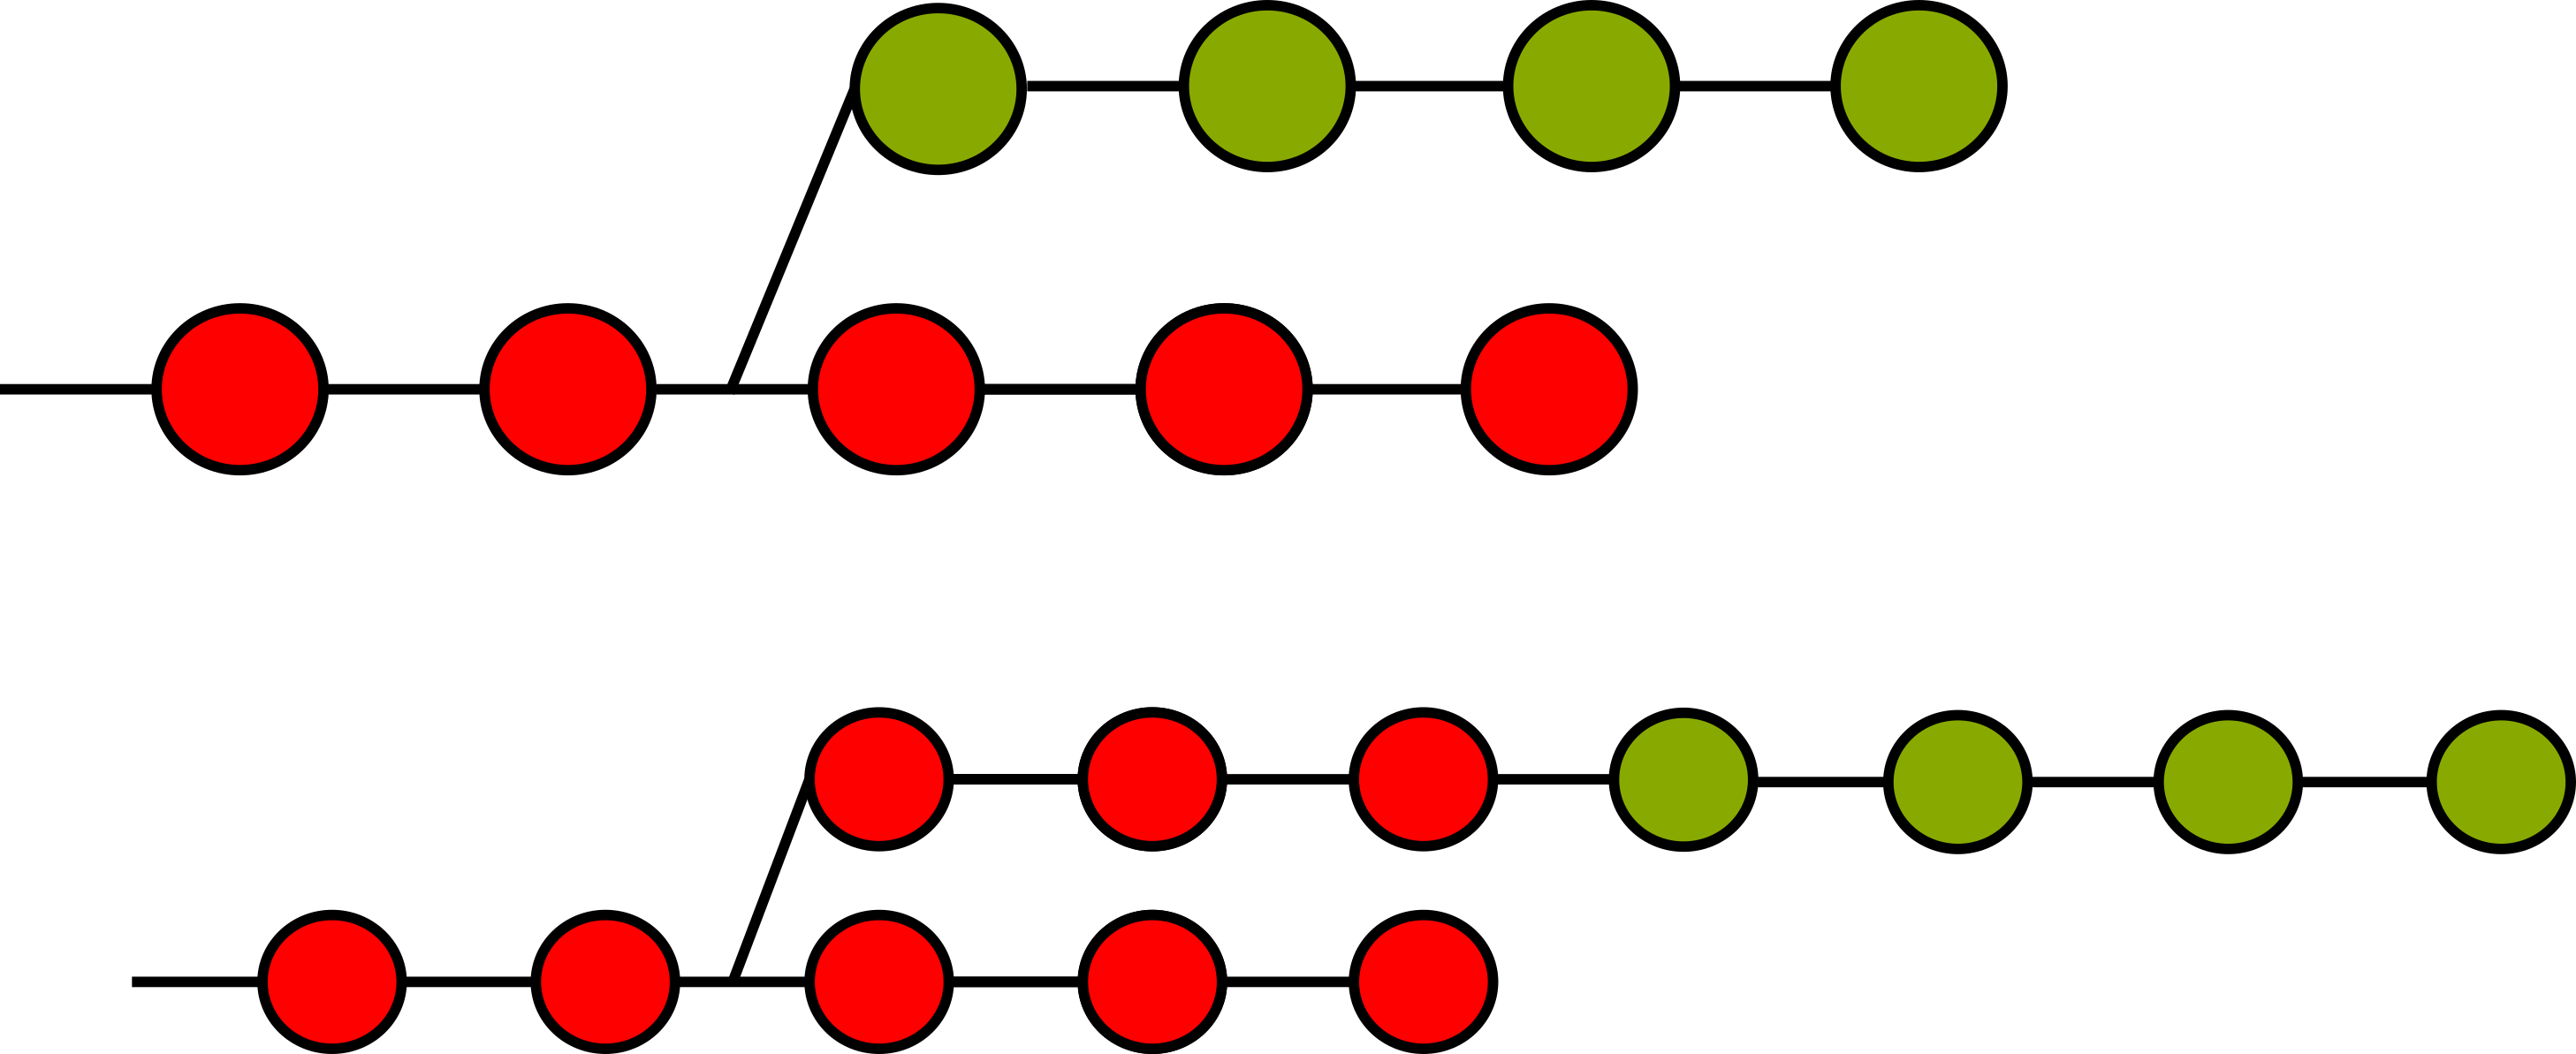
\includegraphics[width=10cm]{images/rebase}
\end{frame}

\begin{frame}{Slučování větví - roubování}
	Větve sloučíme následujícím postupem.
	
	\begin{enumerate}
		\item Přepneme se do zdrojové větve \\
		\texttt{git checkout source-branch}
		\item Naroubujeme zdrojovou větev na cílovou větev \\
		\texttt{git rebase target-branch}
		\item Přepneme se do cílové větve \\
		\texttt{git checkout target-branch}
		\item Sloučíme zdrojovou větev do cílové\\
		\texttt{git merge source-branch}
	\end{enumerate}
\end{frame}

	\begin{frame}{Rozdíl mezi prorůstáním a roubováním}
		Prorůstání má následující vlastnosti, které roubování nemá:
		\begin{itemize}
			\item zachování pořadí commitů
			\item \textbf{merge commit} v historii
		\end{itemize}
	Použití jednotlivých strategií závisí na osobních či projektových preferencí.
	\end{frame}

	\begin{frame}{Konflikt slučování (merge conflict)}
	Jestliže se obsah dvou větví liší ve stejném místě, potom při slučování vznikne \textbf{konflikt}. V takovém případě se Git chová velmi konzervativně a \textbf{nedovolí sloučení}, dokud konflikt nebude vyřešen.
	\end{frame}

	\begin{frame}{Důvod konfliktu}
	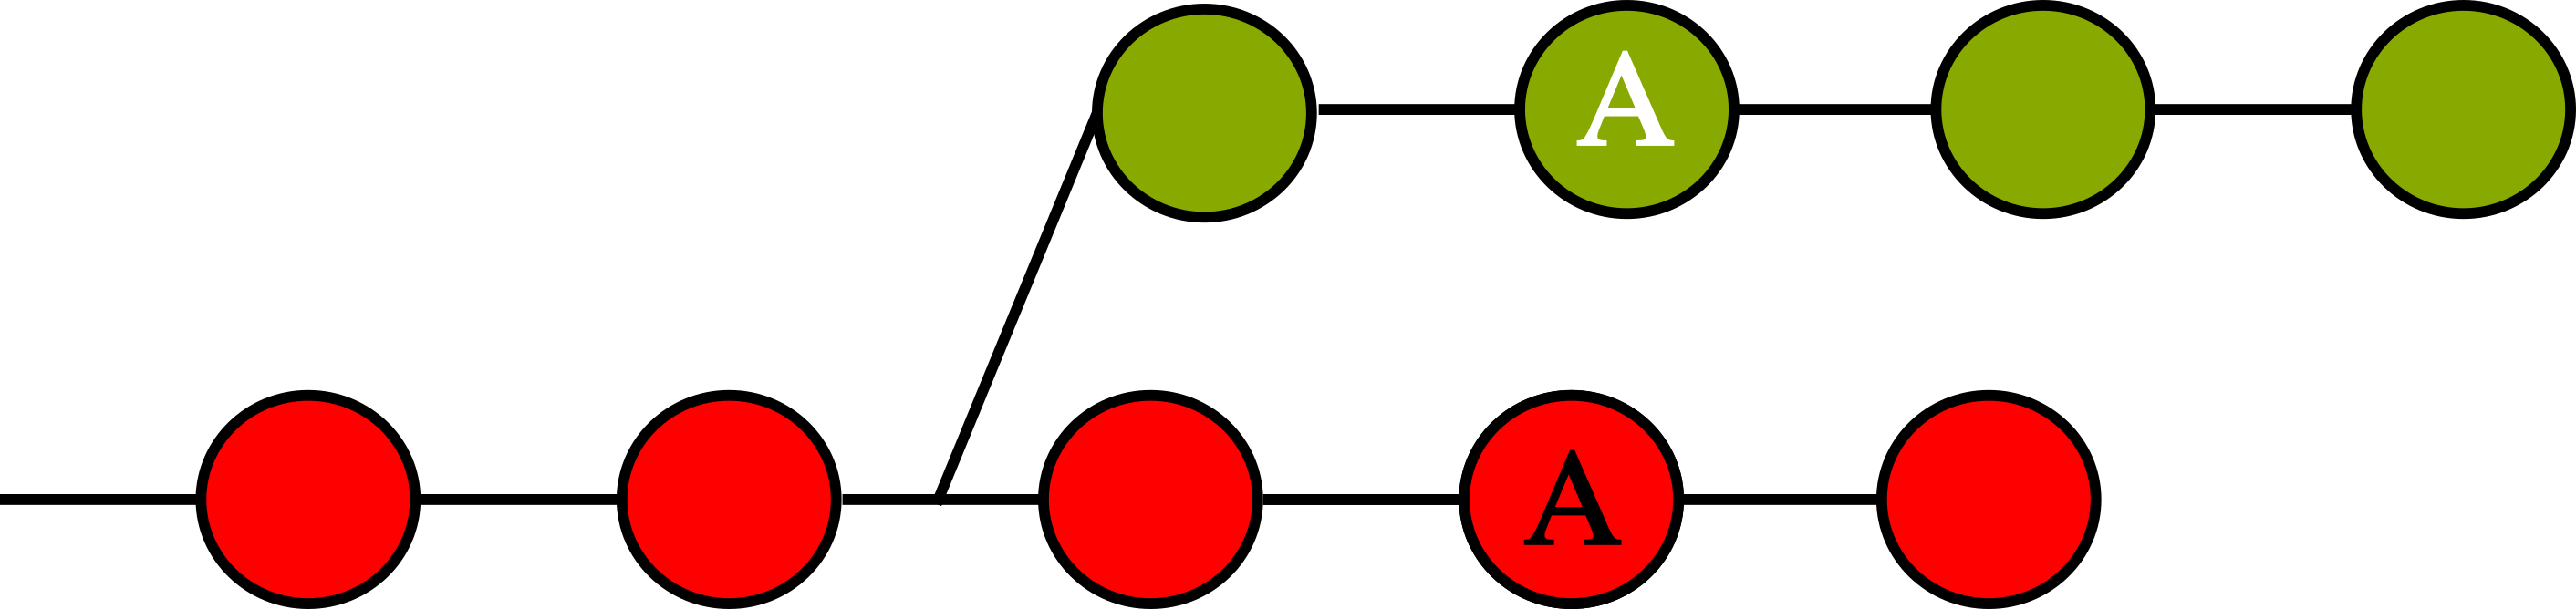
\includegraphics[width=10cm]{images/conflict}
	\end{frame}
	

	\begin{frame}{Řešení konfliktu}
		Kdykoliv Git hlásí konflikt při provádění slučovacího příkazu (merge, rebase), je potřeba jej nejprve ručně vyřešit, než můžeme větve sloučit.
		\begin{enumerate}
			\item Otevřeme soubor, ve kterém je konflikt.
			\item Najdeme řádek \texttt{<\,<\,<\,<\,<\,<\,< HEAD}
			\item Najdeme řádek \texttt{>\,>\,>\,>\,>\,>\,>}
			\item A mezi nimi najdeme řádek \texttt{=======}
			\item Všechno směrem nahoru je obsah původní větve.
			\item Všechno směrem dolů je obsah nové větve.
			\item Upravíme soubor tak, aby v něm zůstalo pouze to, co chceme. Uložíme soubor.
		\end{enumerate}
	\end{frame}

	\begin{frame}{Řešení konfliktu}
	
	\begin{enumerate}
		\item Řekneme gitu o změnách\\
		\texttt{git add corrected-file}
		\item Můžeme pokračovat ve slučování \\
		\texttt{git merge -\,-continue} nebo \texttt{rebase -\,-continue}
		\item Pokud se objeví další konflikt, vyřešíme jej a všechny další konflikty také.
		\item Po vyřešení všech konfliktů obsahuje cílová větev změny ze zdrojové větve.
	\end{enumerate}
	\end{frame}

	\begin{frame}{Smazání větve}
		Nepotřebnou větev můžeme smazat. Git nikdy nesmaže větev ze serveru, i když ji smažeme lokálně. Pro smazání ze serveru musíme použít jiný příkaz.
	\begin{itemize}
		\item Pro smazání sloučené větve. Git varuje, pokud větev není sloučená.\\
		\texttt{git branch -d branch-to-delete}
		\item Pro smazání jakékoliv větve \\
		\texttt{git branch -D branch-to-delete}
		\item Smazání větve na serveru \\
		\texttt{git push origin -\,-delete branch-to-delete}
	\end{itemize}
\end{frame}

	\begin{frame}{Přidáváme k již uzavřenému commitu}
	\begin{itemize}
		\item \texttt{git commit -\,-amend}
		\item upravíme commit message
		\item \texttt{git push} hlásí chybu $\ldots$ proč?
	\end{itemize}
	\end{frame}

	\begin{frame}{Důvod konfliktu}
	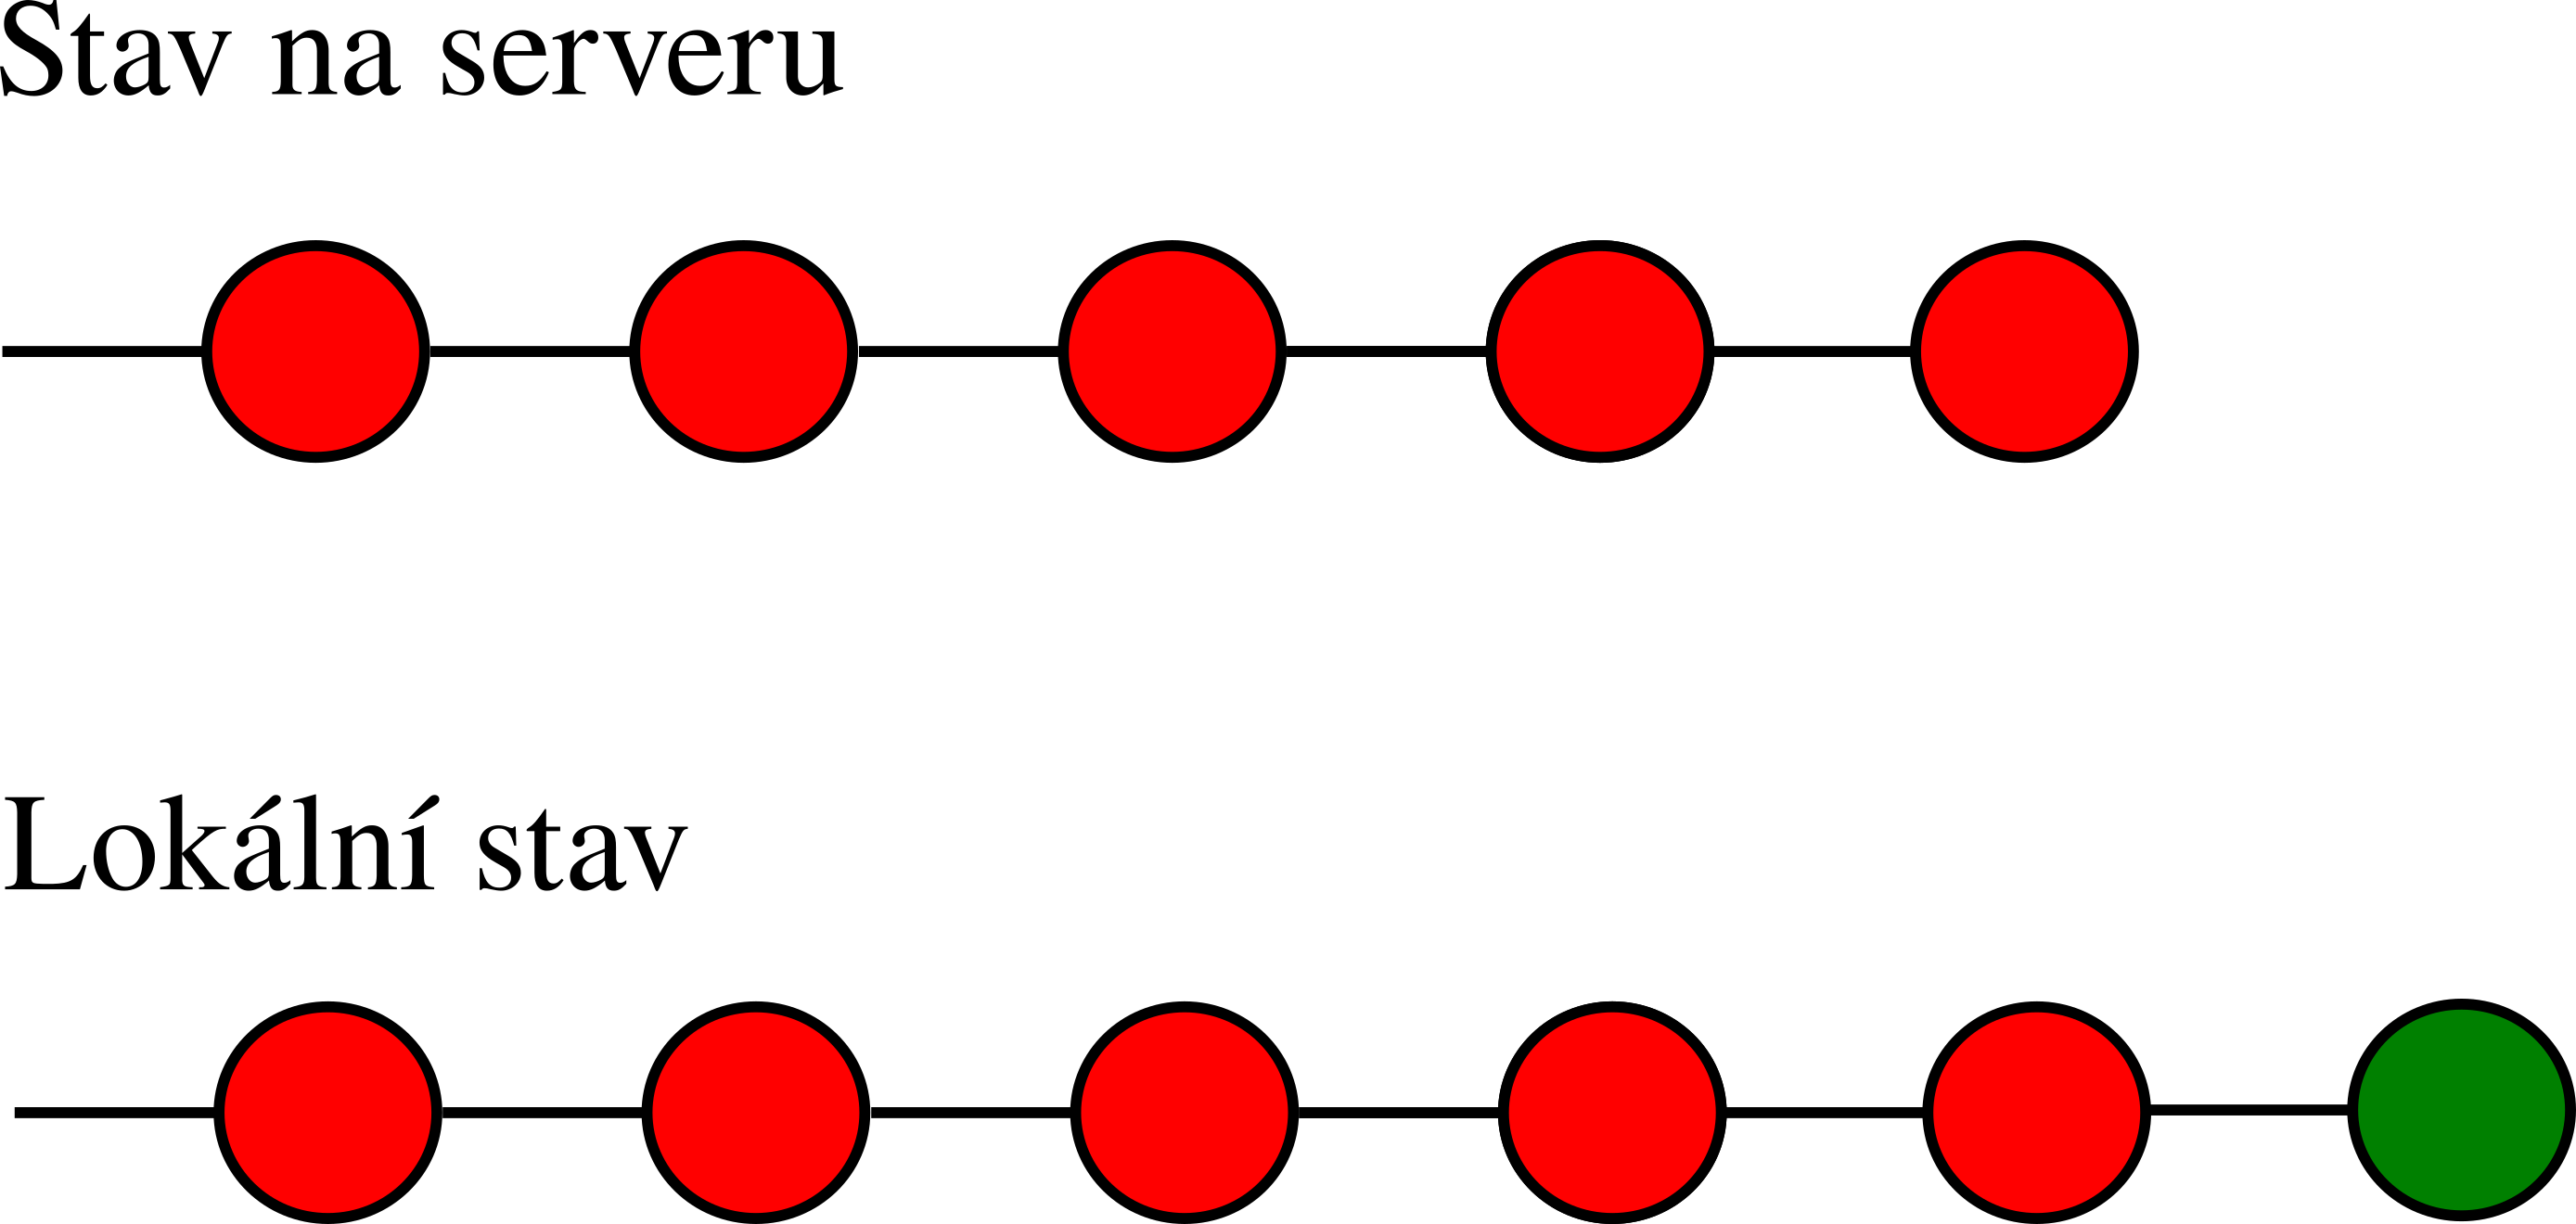
\includegraphics[width=10cm]{images/amend}
	\end{frame}

	\begin{frame}{Vynucení změny}
		Pokud jsme si jisti, že naše lokální větev má správnou verzi a na serveru je verze nesprávná, můžeme Gitu přikázat, aby serverovou verzi přepsal verzí lokální.
		
		To může mít ale velké dopady na synchronizaci a proto to většinou děláme \textbf{pouze u soukromých větví}.
	\begin{itemize}
		\item \texttt{git push -\,-force}
	\end{itemize}
	Vzdálená větev bude bez dalšího přepsána lokální variantou.
	\end{frame}

	\begin{frame}{Konflikty po forcepush}
	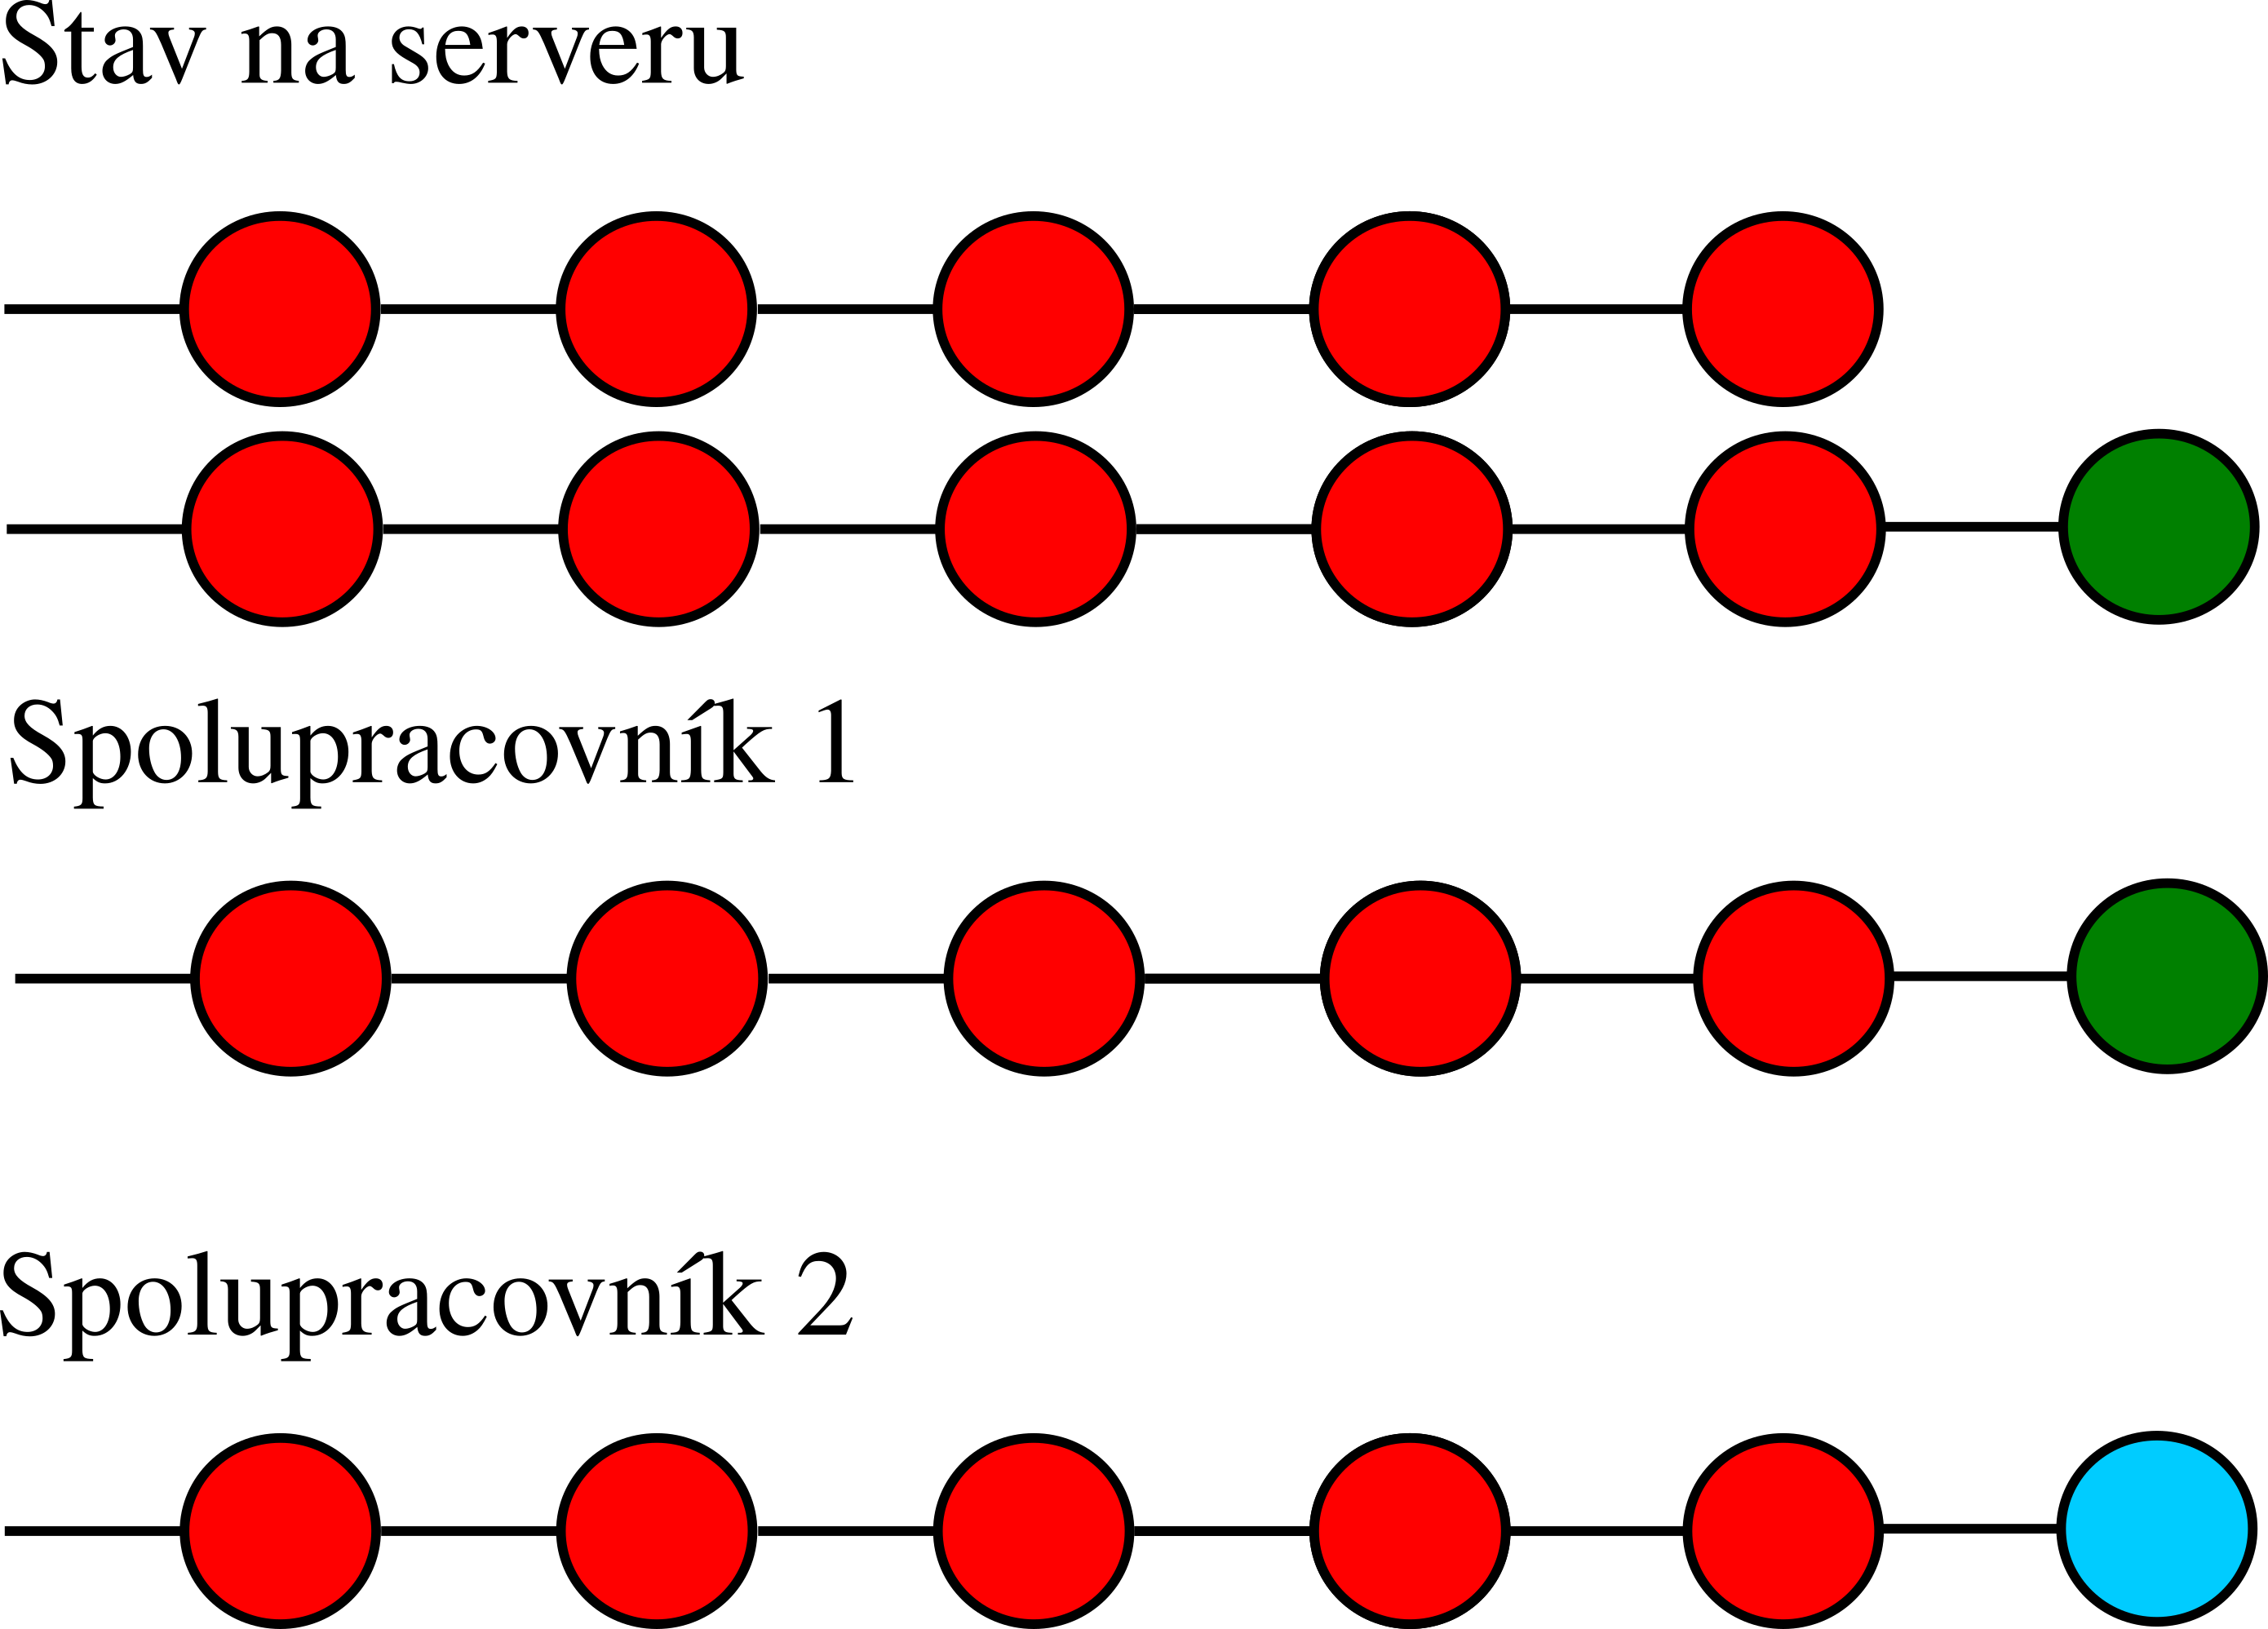
\includegraphics[width=10cm]{images/forcepush}
	\end{frame}


	\begin{frame}{Měníme historii -- interaktivní rebase}
		Při \textbf{interaktivním} rebase můžeme upravit historii commitů podle toho, jak potřebujeme:
	\begin{itemize}
		\item změnit commit message
		\item spojit několik commitů dohromady (squash)
		\item zahodit některé commity
		\item změnit strukturu repozitáře
	\end{itemize}
	Jakékoliv změny v historii větve \textbf{vyžadují forcepush} a mohou mít neblahé důsledky na všechny lidi, kteří na větvi pracují.
	\end{frame}

	\begin{frame}{Git jako stroj času}
		Vzhledem k tomu, že si Git pamatuje všechny změny, které kdy ve větvi nastaly, tak je možné například 
		\begin{itemize}
			\item porovnat dva body v čase nebo dvě větve
			\item vymazat přítomnost, vrátit se do historie, a začít znovu
			\item vrátit se do historie a vytvořit větev v místě návratu
		\end{itemize}
	\end{frame}

	\begin{frame}{Porovnání dvou verzí}
		Pomocí \texttt{git diff} si můžeme zobrazit rozdíly mezi dvěmi prvky.
		\begin{itemize}
		\item \texttt{git diff hash1 hash2}
		\item \texttt{git diff origin/branch branch}
		\item \texttt{git diff branch1:file1 branch2:file1}
	\end{itemize}
\end{frame}

\begin{frame}{Smazání současnosti a návrat do minulosti}
	Můžeme si vybrat, na který commit se vrátíme a veškerý novější obsah zahodíme.
	\begin{itemize}
		\item \texttt{git reset 123456} (soft reset)
		\item \texttt{git reset -\,-hard 123456} (hard reset)
	\end{itemize}
	\textbf{Hard reset} také navrátí stav souborového systému na stav dotyčeného commitu. \textbf{Soft reset} pouze posune ukazatel \textit{HEAD}, ale obsah souborů zůstane nezměněn.
	
	\textbf{Pozor! \texttt{git reset} mění historii větve a porušuje její kontinualitu.}
\end{frame}

\begin{frame}{Smazání současnosti a návrat do minulosti}
	Pokud chceme smazat nějaký commit, ale zároveň nechceme, aby se změnila historie větve (například na \textit{master} větvi), můžeme commit tzv. \textbf{revertnout}.
	
	To vytvoří nový commit, jehož obsah změní obsah větve na stav, jako by odstraňovaný commit ve větvi vůbec nebyl.
	\begin{itemize}
		\item \texttt{git revert 123456} 
	\end{itemize}
	Je potřeba si uvědomit, že čím v historii vzdálenější commit chceme revertnout, tím více konfliktů budeme možná muset řešit. Někdy je tedy daleko lepší provést změny ručně a znovu je commitnout.
\end{frame}

\begin{frame}{Návrat do minulosti a vyvětvění z toho místa}
	Někdy bychom se chtěli vrátit do minulosti a zkusit jinou cestu, ale zároveň si chceme uchovat, to, co už máme. 
	\begin{itemize}
	 \item Můžeme se tedy vrátit k určitému commitu \\ \texttt{git checkout
		 123456} 
	 \item A z toho místa vyvětvit novou větev \\ \texttt{git checkout -b newbranch}
	\end{itemize}
	Pak budeme mít jak původní větev se všemi změnami, tak původní větev s novými změnami.
\end{frame}

	\begin{frame}{Jak se vyhnout problémům -- dobrá praxe}
	Problémům s konflikty se nelze vyhnout, ale lze je podstatně snížit, když dodržíme následující:
	\begin{itemize}
		\item pravidelně aktualizujeme master větev a rebasujeme na ni
		\item každý pracuje ve své vlastní větvi
		\item než commitnu změny, vždycky předtím pullnu
		\item nikdy neměníme obsah a historii master větve
		\item commitujeme menší celky, případný konflikt se řeší \textbf{hned}
	\end{itemize}
\end{frame}

\begin{frame}{Proč nejde pullnout nebo pushnout?}
	Někdy se, kvůli různým zásahům do historie repozitáře, odlišuje lokální od vzdálené větve. Potom Git \textbf{nedovolí} aktualizovat lokální větev pomocí \texttt{git pull}.
	
	Mezi nejčastější důvody patří
	\begin{itemize}
		\item lokální větev je napřed před vzdálenou větví 
		\item mezi lokální a vzdálenou větví je konflikt 		
		\item historie commitů se mezi větvemi liší
	\end{itemize}
	Někdy se Git pokusí situaci napravit sám, většinou je nutný zásah z venčí. 
\end{frame}

\begin{frame}{Lokální větev je novější než vzdálená}
	\begin{itemize}
		\item \texttt{git push}
	\end{itemize}
\end{frame}

\begin{frame}{Lokální a vzdálená větev mají jinou historii}
	Toto se stane, když někdo provede nějaké změny historie na dotyčné větvi. Většinou by to neměl být problém, protože předpokládáme, že vzdálená větev je správná. V~tom případě stačí naši větev resetnout podle vzdálené větve.
	\begin{itemize}
		\item \texttt{git fetch origin}
		\item \texttt{git reset --hard origin/branch}
	\end{itemize}
\end{frame}

\begin{frame}{Lokální a vzdálená větev mají jinou historii}
Když mám nějaké lokální commity, které na vzdálené větvi nejsou a o které nechceme přijít. V tom případě
	\begin{itemize}
		\item Najdeme společný commit a naši větev softresetneme na tento commit. \\ \texttt{git reset 12fg56}
		\item Všechny naše úpravy odložíme do úschovny \\
		\texttt{git stash}
		\item Potom resetneme na vzdálenou větev\\
		\texttt{git reset -\,-hard origin/branch}
		\item Aplikujeme změny z úschovny\\
		\texttt{git stash apply}
		\item Commitneme a pushneme.
	\end{itemize}
\end{frame}

\begin{frame}{Vyzobnutí jednoho commitu do jiné větve.}
	Někdy můžeme mít v jedné větvi zajímavý commit, který chceme použít v jiné větvi, která se ale jinak zásadně liší. Takový commit si můžeme vyzobnout jako \textit{třešničku na dortu}.
	\begin{itemize}
		\item \texttt{git checkout branch-to-keep}
		\item \texttt{git cherry-pick commit}
		\item Vyřešíme případně konflikty.
	\end{itemize}
\end{frame}

\begin{frame}{Otázky?}
	Kdo má otázky, ať se zeptá teď \ldots{}
	
	\vspace{15pt}
	
	\ldots{} nebo navždy pomlčí.
\end{frame}

\begin{frame}{}
	Děkuji za pozornost!
\end{frame}



\end{document}
